\documentclass[a4paper,twocolumn]{article}
\usepackage{color,graphicx}
\usepackage{natbib}

\bibliographystyle{plainnat}
\title{Extending reinforcement learning to Tetris \\ Short Paper}
\author{Donald Carr\thanks{Sponsored by Microsoft, Telkom, Thrip, Comverse, Verso and Business Connexion} \\ Department of Computer Science \\ Rhodes University \\ Grahamstown 6139,South Africa \\ g02c0108@campus.ru.ac.za}
\begin{document}
\maketitle
%\tableofcontents
%\listoffigures
%\listoftables

\begin{abstract}
This paper discusses the reduction of the Tetris state space in order to satisfy the pragmatic storage and computational requirements of tabular reinforcement learning. A Sarsa based agent is implemented, and shows convincing learning when using simplified Tetris blocks.
\end{abstract}

\section{Introduction}

Reinforcement learning is a branch of artificial intelligence that focuses on achieving the learning process in the course of a digital agents lifespan. This entails giving the agent perception of its circumstances, a memory of previous events and rewarding it on account of its actions in the context of a rigid, predefined reward policy. 

Reinforcement learning has been successfully utilised to solve a diverse range of problems, although it has had limited success with large problems \citep{keepaway}. This is due to a state space explosion that inevitably occurs as the agent tries to remember every single variation in increasingly complex problems.

Suggestions for solving this problem have taken many forms. Tesauro \citep{tdgammon} created a hybrid agent in his backgammon game that was comprised of a neural network whose weighting was progressively tuned by reinforcement learning. \cite{kurt} suggested implementing a tree structure which adds nodes as they are encountered, thereby skirting the problem. A common approach in reinforcement learning is function approximation, where rather then giving the agent a discrete memory, a function is gradually developed that takes a state as an input and issues back a value. This removes the need for a one to one relationship, and thereby removes the problem. 

Tetris is a well established game, and has been thoroughly investigated by both the mathematical and artificial intelligence communities. Although conceptually simple, it is NP-complete \citep{hardtet} and any formalised optimal strategy would be incredibly contentious. Tetris is found in a variety of forms, and this paper is limited to Tetris as defined by \cite{tetstand}. Certain sequences of tetrominoes guarantee the death of the agent, and therefore every game of Tetris invariably ends \citep{mathproof,losetetris}. This episodic behaviour makes comparing subsequent games possible as the agents performance can be gauged by the number of rows completed in the course of a game.

Reinforcement learning has been successfully applied to a very reduced version of Tetris \citep{melaxtetris,yaeltetris}, and less successfully applied to a complete version of Tetris \citep{kurt}. 

\section{Tetris}

The player is handed a tetromino uniformly drawn from the limited range of predefined tetrominoes shown in figure \ref{fig:fulltet}. Each of these tetrominoes is defined as a static relationship between the constituent blocks, allowing the same Tetromino to exist in any of its rotations. The game occurs within a well which is defined by a grid of blocks, with dimensions twenty deep by ten wide. The tetrominoes enter at the top and are set in a fixed position upon hitting the first obstruction they encounter, which is the bottom of the well failing all else. When a row is completely filled it vanishes and the player is rewarded.

\begin{figure}[h]
\centering
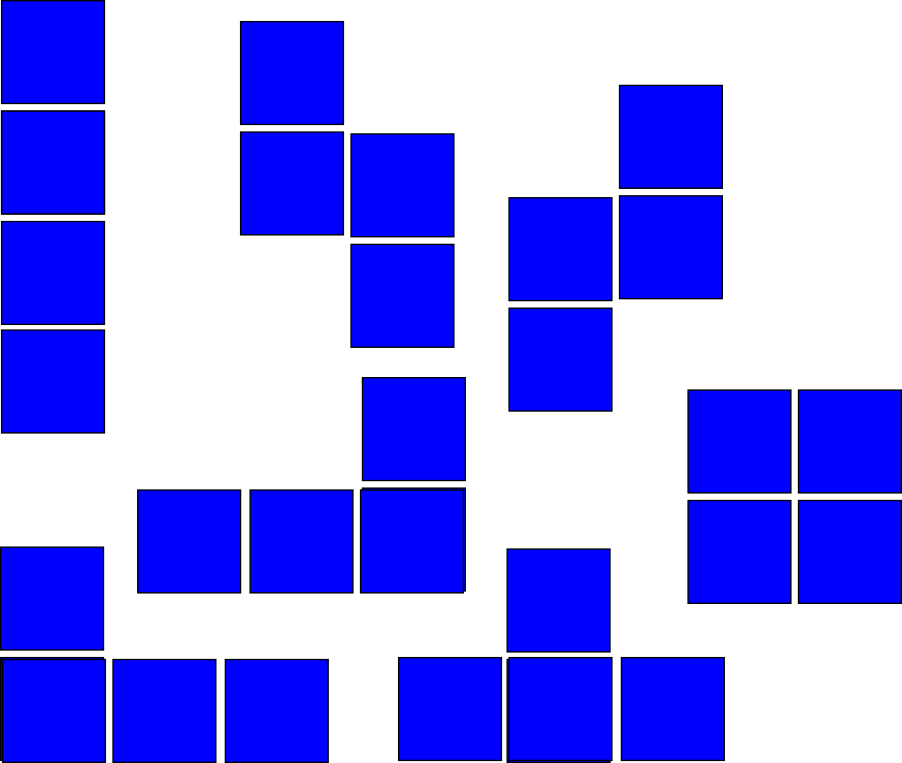
\includegraphics[width=1.5in]{fullblocks.png}
\caption{The classic set of Tetris tetrominoes}
\label{fig:fulltet}
\end{figure}
  
\section{The Tetris state space}

Traditional reinforcement learning uses a tabular value function, which has a one to one relationship between states and values. Since the Tetris well has dimensions twenty blocks deep by ten blocks wide, there are 200 block positions in the well that can be either occupied or empty.

\begin{figure}[h]
\centering
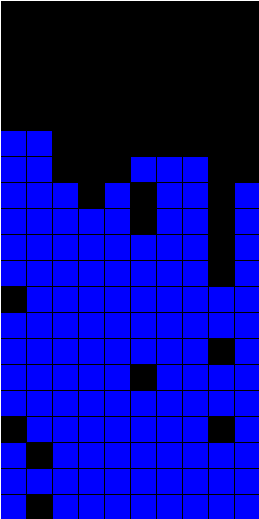
\includegraphics[width=0.8in]{fullwell.png}
\caption{The compete Tetris well}
\label{fig:fullwell}
\end{figure}

\begin{eqnarray}
\textrm{State Space} & = & 2^{200} 
\end{eqnarray}

This is an unwieldy number and since a value would have to be associated with each state, this representation is completely non-feasible. By considering the game from a human perspective, we considered some practical reductions in state space. 

\subsubsection*{Assumption 1}

The position of every block on screen is not a consideration that is factored into every move. We only consider the contour of the well when making decisions. We limit ourselves to merely considering the height of each column.

\begin{figure}[h]
\centering
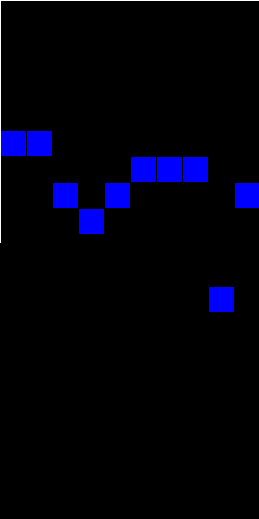
\includegraphics[width=0.8in]{heightwell.png}
\caption{Height based Tetris well}
\label{fig:heightwell}
\end{figure}

\begin{eqnarray}
\textrm{State Space} & = & 20^{10} \approx 2^{43}
\end{eqnarray}

\subsubsection*{Assumption 2}

The height of each column is fairly irrelevant except perhaps when the height of a column starts to approach the top of the well. Ignoring this for the time being, the importance lies in the relationship between successive columns, rather then their isolated heights.

\begin{figure}[h]
\centering
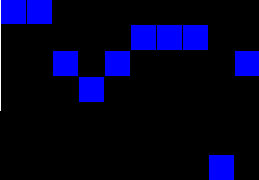
\includegraphics[width=0.8in]{diffheightwell.png}
\caption{Height difference based Tetris well}
\label{fig:diffheightwell}
\end{figure}

\begin{eqnarray}
\textrm{State Space} & = & 20^{9} \approx 2^{39}
\end{eqnarray}

\subsubsection*{Assumption 3}

Beyond a certain point, height differences between subsequent columns are indistinguishable. A human will not adopt different tactics when the height difference between two columns advances from nineteen to twenty. We could either cap the maximum height differences, or start separating the heights into fuzzy sets as the height differences increase past certain thresholds. We cap the maximum height difference between wells as $\pm$ 3, and round all height differences outside of this range down to $\pm$ 3. The agent will therefore generalise for any height difference greater then 3. Since only the straight tetromino can span a height difference of 3, and this tetromino can span any height difference, this assumption seems fair to make. 

\begin{figure}[h]
\centering
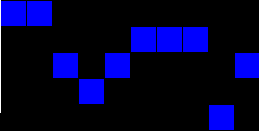
\includegraphics[width=0.8in]{capdiffheightwell.png}
\caption{Capped height difference based Tetris well}
\label{fig:capdiffheightwell}
\end{figure}

\begin{eqnarray}
\textrm{State Space} & = & 7^{9} \approx 2^{25}
\end{eqnarray}

\subsubsection*{Assumption 4}

The largest tetromino is four blocks wide. At any point in placing the tetromino, the value of the placement can be considered in the context of a subwell of width four. These subwells could then be reproduced across the extent of the full well.

\begin{figure}[h]
\centering
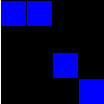
\includegraphics[width=0.8in]{reducedwell.png}
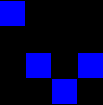
\includegraphics[width=0.8in]{reducedwell2.png}
\caption{Capped height difference based Tetris subwells}
\label{fig:redwell}
\end{figure}

\begin{eqnarray}
\textrm{State Space} & = & 7^{3} = 343 \approx 2^{8}
\end{eqnarray}

\subsubsection*{Assumption 5}

Since the game is stochastic, and the tetrominoes are uniformly selected from the tetromino set, the value of the well should be no different to its mirror image.

\begin{figure}[h]
\centering
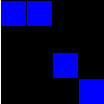
\includegraphics[width=0.8in]{reducedwell.png}
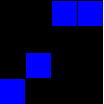
\includegraphics[width=0.8in]{mirrorwell.png}
\caption{Mirror identical states}
\label{fig:mirrorwell}
\end{figure}

\begin{eqnarray}
\textrm{State Space} & = 175
\end{eqnarray}

We now have a much reduced statespace, which we hope will neither limit the player nor appreciably steer its policy. The implications of the assumptions should be considered before we progress.

Assumption 1 discards all information about the subsurface structure of the well. The initial representation can be perceived to store the location of every hole in the structure. The agent will therefore be oblivious to any differences between transforming to a said contour and the same contour with spaces beneath the surface. The existing holes are not important, but we may wish to include a penalty for the holes introduced during a state transition.
Assumption 2 introduces no obvious evils.
Assumption 3 removes the agents ability to distinguish between extremes in height differences.
Assumption 4 removes the global context in which the agent functions, and restricts his view to each individual transition. We may need to dynamically reestablish the context in which he is functioning.
Assumption 5 reduces the state space in a non-simple fashion. The mirrored states are still allocated space, but are never explored, removing the computational burden they represent. 

\section{Implementation}

Only the tetromino currently allocated to the agent is considered during each move.

When the value functions values are initialised they are assigned an unrealistically large initial value. This is referred to as optimistic learning, and results in the agent attempting every transition, and sticking with those that disappoint it least.

The value of the prospective states was ascertained by using afterstates \citep{suttonbarto}. The agent drops the given tetromino in each and every possible orientation and each resulting final configuration is hashed to a single value.  Each configuration is hashed twice, from both directions in order to implement the mirror symmetry reduction. The smallest value is then always selected. Each of these hash codes is compared with each member of an array of existing hash codes. If the hash code has not been seen before, it is included the array, otherwise it is redundant and therefore discarded. Each hash code is used to access a value associated with that configuration in the value function.

All the afterstate manipulations occur within a virtual game, that is used exclusively by the agent and is separate and distinct from the real game the agent is confronted with.

The agent individually combines these values with any immediate reward that is associated with that particular state transition. The agent now has an array of unique transitions and the total reward associated with them.

If the agent is exploiting, it selects the array element with the largest reward associated with it. If the agent is exploring using $\epsilon$-greedy methods, it selects randomly within this array a small percentage of the time. Given multiple elements with the shared largest value, the agent selects randomly amongst them. If the agent is exploring intelligently through the softmax approach \citep{suttonbarto}, the transitions are selected with a probability proportional to their associated reward.

After selecting a transition, the value of the current state is updated. The updated value is a combination of the reward received in the transition, the value of the destination state and the existing value. The relation between these factors is described by standard Sarsa \citep{suttonbarto}.

\begin{eqnarray}
Q_{t+1}(s) = Q_{t}(s_{t}) + \alpha (r_{t+1} + \gamma Q_{t}(s_{t+1}) - Q_{t}(s_{t}) )
\end{eqnarray}

The agent is given a constant $\alpha$ value of 0.2, and a $\gamma$ value of 0.8 as these values were empirically ascertained to inspire decent performance in a much reduced version of Tetris. \footnote{The author reproduced the results of \cite{melaxtetris,yaeltetris}}

Determining an unprejudiced reward function, conducive to rapid learning, is a non-trivial task.

  A negative reward for an increase in height \citep{melaxtetris,yaeltetris} assumes that height should be minimised and directs the agents policy. This circumvents the point of Tetris, which is to maximise the number of rows completed and therefore maximise the agents lifespan. Although there is a strong correlation between keeping the height down and surviving, an optimal policy may involve defying this basic tenet. By rewarding the agent 100 points for each row completed, he is driven to completing rows without being coerced into a predetermined approach.

  Unless the agent is punished for death, he remains oblivious to its existence and will chance upon it at the end of every game. In order to avoid this we decided to punish the agent 100 points for dying.
  
     The numerical relationship between these component rewards is not obvious, and observation of the agents response to variation in these rewards was used to guide the reward values.
  
\section{Reduced Tetris}

\begin{figure}[h]
\centering
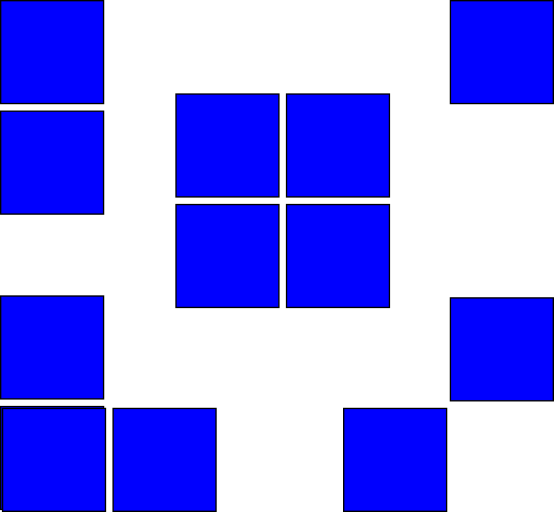
\includegraphics[width=1.5in]{reducedblocks.png}
\caption{The set of reduced tetrominoes}
\label{fig:redtet}
\end{figure}

In order to verify that the agent is learning within the perceptive framework of the reduced state space we implemented a reduced Tetris. This operated within a twenty by four well. We used a reduced set of tetrominoes, shown in figure \ref{fig:redtet}, in order to simplify the learning process and establish whether our state reductions would still permit active learning on the part of the agent. 

\begin{figure}[h]
\centering
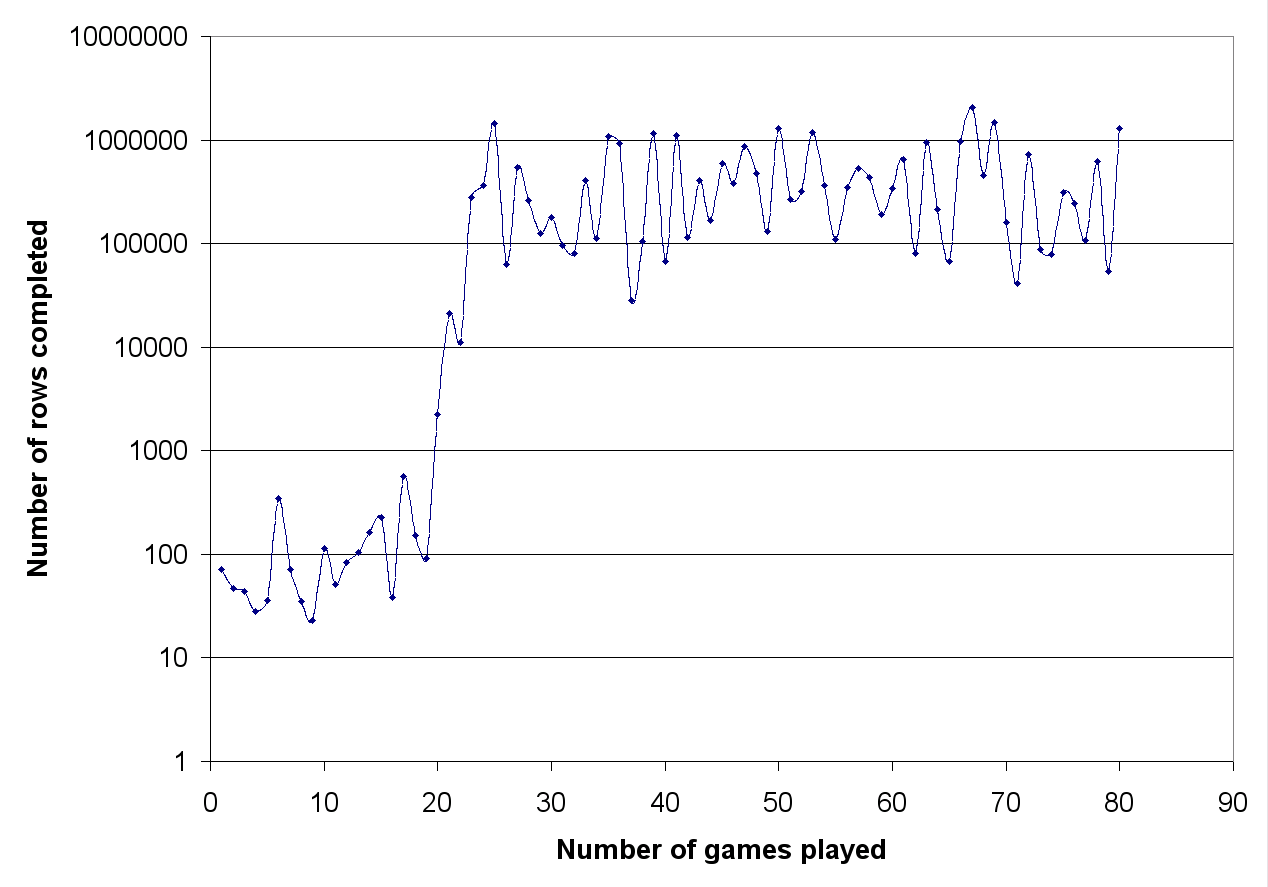
\includegraphics[width=3in]{reducedresults.png}
\caption{Numbers of rows completed versus number of games played by reduced agent}
\label{fig:redgenius}
\end{figure}

These results are achieved by setting the agent to exploit his knowledge from the offset and relying on the optimistic initial values for encouraging exploration. It is evident from figure \ref{fig:redgenius} that after about 50 games the agent has discovered the optimal policy. 

These results are incredible although possibly misleading, since the dimensions of the well are so similar to those of the pieces. Since the dimensions are so similar, the rewards are very frequent and dwarf the long term values, thus putting the agent is in a position to constantly reap reward. The value of reinforcement learning comes from its ability to sacrifice short term rewards in order to gain a greater long term reward. As the well widens the agent has to increasingly consider its long term prospects.

\begin{figure}[h]
\centering
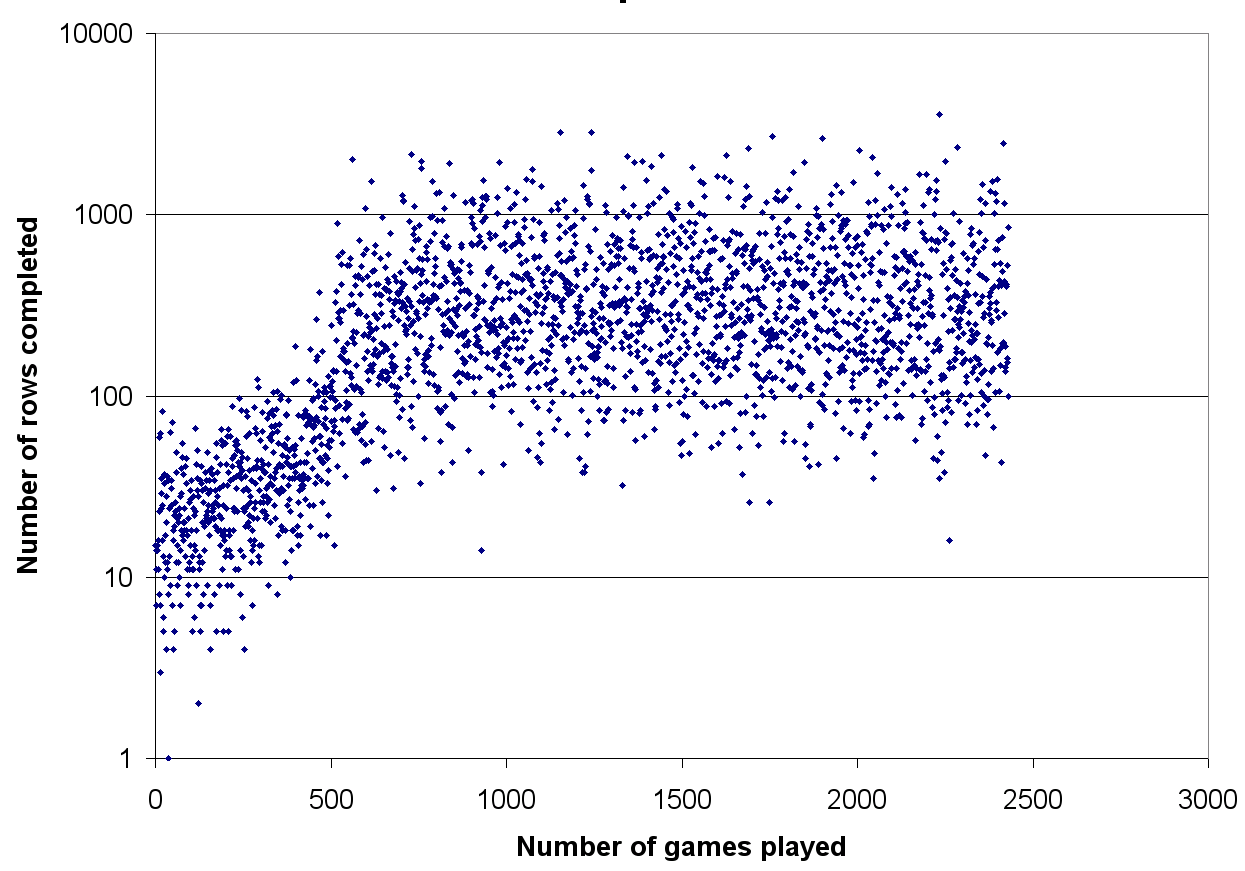
\includegraphics[width=3in]{width5results.png}
\caption{Numbers of rows completed versus number of games played by reduced agent, width 5}
\label{fig:5width}
\end{figure}

It is apparent that the results drop off drastically as the agent has to rely more heavily on the the anticipatory values. This is unsettling.

\section{Full Tetris}

The reduced Tetris algorithm is extended by dividing the full game into strips. At the afterstates level, the agent considers a well of width four and attempts all the possible translations and orientations of the tetromino in that well. The virtual well is shifted across the real well by one block width, and the agent repeats his transition discovering procedure. This is repeated for every single well of width four within the full well.

\begin{figure}[h]
\centering
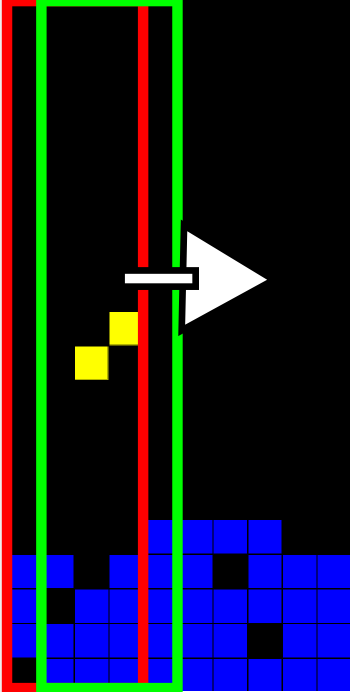
\includegraphics[width=1.1in]{decomposedwell.png}
\caption{Reduced well progression across the full well }
\label{fig:6width}
\end{figure}

Since there is overlap in-between translating the well one step right, and shifting the agent one step left, there are multiple values discovered for each unique transition, in the context of different wells. We chose to average these values, in order for the value of the transition to convey its broad impact on the agent.

The agent is trained in the well of width four, and its value function is subsequently saved. The agent is re-instantiated with the full well, of width 10, and its ability to learn is disabled. The aforementioned value function is loaded and guides the agent is evaluating the value of a certain transition. These transitions are idealised and created around a well of width four, and we insert a weighting which renders height inversely proportional to weighting. This does not overwrite the value function, but encourages the agent to broaden out, rather then building up the well. Since there is a disparity between the reward associated with a transition in the reduced well and the reward associated with the transition in the full well, a second conceptual game is now required.

We implemented the extended version of the reduced Tetris game, complete with the reduced blockset.  

\begin{figure}[h]
\centering
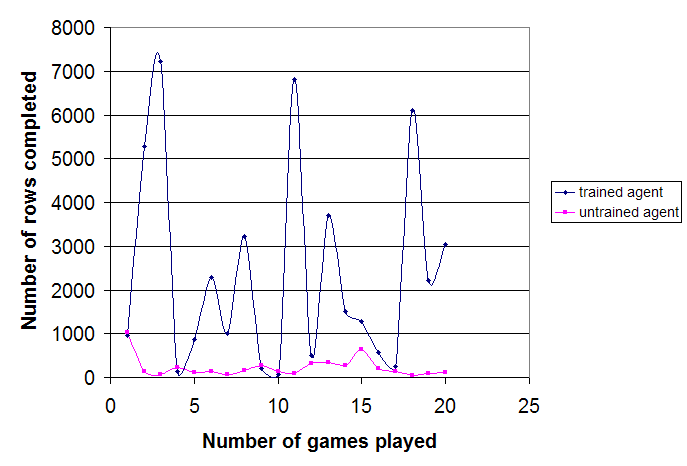
\includegraphics[width=3in]{fullreducedgame.png}
\caption{Results for full Tetris, width 6}
\label{fig:fullgame}
\end{figure}

The results depicted by figure \ref{fig:fullgame} reveal an obvious improvement in the performance of the agent with the inclusion of the trained value function from the reduced player. The performance of the agent is not steady, and varies largely over a short number of games. It must be noted that the agent is not displaying "hunting" \footnote{An oversensitivity to negative feedback, resulting in oscillation around the optimal solution} and that no learning is occurring at this stage, since the agent is merely functioning under the guidance of a static value function.

\section{Considerations}

Attempts at learning in the reduced well with the complete blockset have met with little success. Where as the reduced block set experiences a large number of guiding rewards, and functions well with little concern for the holes it is introducing in the well structure, the complexity of the full block set renders this ignorance infeasible. Dynamically altering the appraisal value of a transition, by incorporating a covered hole introduced factor, has met with little success. In some circumstances introducing a hole has little impact, and at others it can completely negate the value of the transition. 

\begin{figure}[h]
\centering
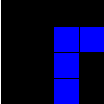
\includegraphics[width=1in]{worthless.png}
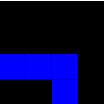
\includegraphics[width=1in]{notworthless.png}
\caption{Contrasting hole inclusion}
\label{fig:diffholes}
\end{figure}

The wells in figure \ref{fig:diffholes} have both introduced the same number of covered holes. They represent two separate transitions, and therefore have differing values associated with them. Altering their respective values by a constant penalty associated with the each introduced hole would not reflect the impact of the holes on the value of the transition. The transition on the left has incremented the height by three, and since it has introduced holes in these rows, it left very little chance of these extra rows being completed. The transition on the right has placed the agent in a position where he is almost certain to complete the row on the next turn, and the height is temporarily incremented by the smallest dimension of the placed tetromino.

\section{Conclusion}

In this paper we developed and justified an approach to reducing the Tetris state space, and successfully implemented a reduced version of the Tetris game. Our proposed method of extending the reduced players experience to a full well was shown to result in a game where learning was evident, but unremarkable. We commented on difficulties encountered in reintroducing the full tetromino set and the likely source of our difficulties. The initial assumptions may have bordered on the optimistic, and over-simplified the informational requirements of a successful agent. Ideally the assumptions can be relaxed to allow more insight to the player, while maintaining a moderately sized state space. There is clear evidence of learning in the reduced game with a state space of 175, and this state space could be considerably expanded to tackle the full game, and still remain feasible.



\bibliography{draftpaper}

\end{document}